\RequirePackage[hyphens]{url}
\documentclass[a4paper,11pt]{article}

\usepackage[british]{babel}
\usepackage{graphicx}
\usepackage{float}
\usepackage{hyperref}

\title{\textbf{Mesh network}\\
  Microcontroller Programming (course 1TE663)\\
  Uppsala University -- Spring 2016}

\author{Per Bergqwist \and Martin Lindstr\"om \and Dennis Pietarinen}

\date{\today}

\begin{document}

\maketitle

\tableofcontents

\newpage

\section{Introduction}
The main goal of this project was to design a protocol to network a
lot of microcontroller using cheap nRF24L01+ modules.  We decided to
develop a self organizing spanning tree mesh network using a
predefined node to be sink.  The sink was connected to a PC which made
the mesh network traffic available through a serial interface. The
result is the possibility to make large, cheap, long-range networks
which are accessible though the internet. Possible use-cases include
remote monitoring and home automation.

\section{Design decisions}
The radio modules support automatic acknowledgment of packets with
optional retransmissions. This enabled us to easily make the
communication between two modules reliable. The auto acknowledgment
feature was used in all communication except for new nodes
broadcasting to connect to the network\cite{nrfDS}.

The radio modules uses GFSK in the 2.4-2.5125Ghz range with support of
data rates from 250Kbps up to a maximum of 2Mbps. The modules uses
1MHz of bandwidth per channel and support 125 different channels. We
decided to use the same frequency for all nodes in the same network to
decrease complexity. This makes all communication within the network
interfere. The radio modules has internal addressing with addresses
consisting of 3-5 bytes. Each module can listen for up to six
addresses at the same time but five of these addresses can only differ
in their last byte. We decided to let the MCU save the addresses and
routing table and only use two of the addresses in the radio
modules. One for broadcast messages and one for unicast messages
directed towards the specified node.

We studied different routing protocols for making a mesh-network,
initially we wanted to have a complete mesh network without a sink but
due to the limited amount of memory available on the chosen MCU we
decided to go for a spanning tree network instead. We figured that
this would make the routing table use less memory since and be less
complex.

Each node keeps a routing table of all nodes located below them in the
network and their corresponding parent node. The sink is the highest
parent. This approach uses memory scaling linearly with the amount of
nodes in the network. The nodes only need to know the route to the
nodes located below themselves.

The address of a node is saved in the microcontrollers EEPROM memory.
This makes it possible to completely shut down a node without it
needing a new address. This decision makes the network only one
address per physical node. We thought about assigning addresses based
on the location of the nodes in the network but this increases the
complexity of the sink node since it would need to keep track of all
active addresses.

\section{Hardware}
Each node consists of one Atmega328P MCU running from the internal
oscillator at 8MHz. It's connected to a nRF24L01+ through the SPI
port. The MCU can be connected to an rs232 adapter to enable debugging
messages to a computer. The sink MCU is connected to an rs232 adapter
to interface with the PC. The nodes accept an input voltage from 2.4v
to 3.6v. Since the NRF24l01+ modules can be run at a minimum of 1.8v
we could potentially run the node at 1.8v but this would require a
lower clock frequency for the MCU\cite{Atmega}.

We built some battery powered nodes that runs from a lithium-ion
battery connected to a 3.3v regulator. The regulator is needed to keep
the input voltage to the radio module below 3.6v.

\section{Software}
The software on the MCU acts as a big state machine. At startup the
MCU is in the unconnected stated. In this state the node is completely
unconnected the network. If a node want's to join a network it needs
to send a broadcast which makes it go into the COLLECTING PARENTS
state. The node will remain in this state until a offer to connect has
been received and a timeout has passed since the last best offer. The
best node is chosen based on hop count. The lower the hop count the
better.

After the timeout has passed a connection attempt is made to the
chosen parent. If this is successful the node will move on to the
next stage, if not the node will try to find a parent again.

Now the node determines if it requires an address or already has one
stored in EEPROM. If an address is required it will ask the sink for a
free address. When the node has a proper address it considers itself
connected to the network.

Now the node will periodically send and receive pings and pongs to and
from the sink node.

When a packet is received that is not destined for this node routing
must be performed. The next hop is calculated and the packet is send
there.

\subsection{Handling packet loss}
When the node tries to send a packet to a another node without
receiving an ACK a couple of resends are performed. If the packet is
not sent successfully after the retries the node is considered out of
range. If this was the nodes parent the node now considers itself
disconnected from the network. It will first try to find a new parent
without alerting its children to reconnect. If this fails it will
continue to try to find a parent but also disconnect its children from
the network.

If the target node is a child the child is removed from the routing
table and this route delete is pushed upwards.

Stats are logged when sending packets to the parent node. These stats
are sent to the sink node as a single byte. This byte should be
divided by 10 and then it represents how many transmissions the node
must perform before a packet reaches the nodes parent.

\subsection{Handling nodes that temporary are out of range}
If a node gets a packet directly from a unknown node that is not in
its routing table the node is added to the routing table, the node is
sent this nodes hop count and the new route is pushed upwards.

If a node get a packet from an unknown node that is relayed through a
direct child the node must ask, through the relaying node, the unknown
node to publish its route upwards.

\subsection{Handling potential route loops}
To speed up the reconnection to the network some design choices were
made so that in some cases route loops can be formed. These loops are
detected when a node receives a packet from itself. The node then
considers itself unconnected so that its children will also do so.

\subsection{Informing old parents of nodes}
When the sink node sees that a node has changed parent the sink send a
route delete to the old parent of the node. This update will then
propagate through all the nodes that had the old route information in
their routing tables.

\subsection{How the sink manages free addresses}
The sink stores information about free addresses in EEPROM.  When the
sink receives a request for a new address it searches after the first
unused address and sends this address back to the requesting node.

\section{Tests}
We measured the current of a non sink node to 13mA at 3.3v. The
current measurement was made from the output of a 3.3v regulator. The
node was put in a always listening state. According to the datasheet
the radio module should consume a maximum of 11mA in listening mode.

We did not to any tests for the power consumption in transmitting
mode.

\begin{figure}[H]
  \includegraphics[width=\linewidth]{EffektMätarSetup}
  \caption{Measuring current with high precision resistor and an oscilloscope}
  \label{fig:Effekt}
\end{figure}

\subsection{Range test}
We measured the maximum range of one hop to 80m in an outdoor
environment when transmitting at 2.52GHz. The maximum indoor range was
measured to 70m in an indoor environment transmitting at 2.52GHz. Both
tests were done with the nodes within line-of-sight.

\section{Interface}

To make it easier to visualizing the network we made a program in Go,
it has a web interface and a backend. The backend reads data from a
connected sink node over the serial interface, it will parse the read
messages and send routing, ping and link quality message over a
websocket to the clients, who are connected via the web interface. The
web interface will display the network as shown in \autoref{fig:web}.

\begin{figure}[H]
  \centering
  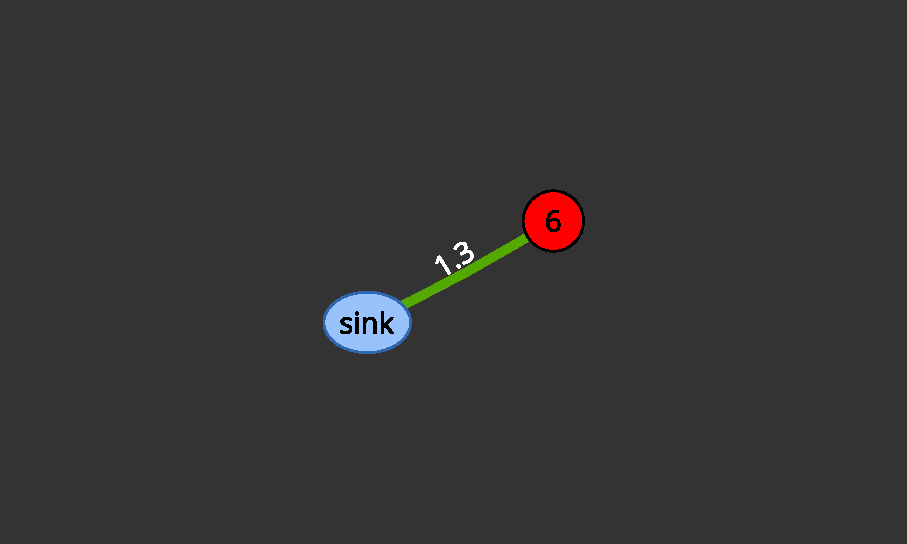
\includegraphics[width=.7\textwidth]{map.pdf}
  \caption{Node 6 is connected to the sink}
  \label{fig:web}
\end{figure}

\section{Discussion}
The implementation behaves as expected and has proved to heal itself
if case of disconnection of routing nodes.

The codes occupies about 8Kb of flash memory and under 700B of ram.
This makes it possible to add more code for gathering sensor data and
possibly interfacing with actuators.

In it's current state the MCU will have to poll the radio module for
new data but it's possible to make the code interrupt driven.

\section{Future work}
The code could be made interrupt driven by the use of the interrupt
pin on the radio modules. This would make the nodes faster at reacting
to events from the radio.

We would like to add some security to the network. Since we are using
wireless signals we are broadcasting all traffic in clear text. As a
start we could implement an AES engine to provide confidentiality of
the network traffic. After this is done we might try to add defense
against replay attacks.

Another useful feature would be to implement support for sleeping
nodes. These nodes would only be powered on at certain intervals to
save energy. The idea is to have these nodes at the edge of the
network so they do not have to route any traffic. As the code works
now these nodes will have to register themselves on the network
everytime they wake up.

The internet interface would be better if the user could send commands
into the network. At the current state we can only get information out
from the network but send any commands.

\begin{thebibliography}{2}

\bibitem{nrfDS}
  Nordic Semiconductors. "\emph{nRF24L01 Product Specification}". [Online]. Available: \url{http://www.nordicsemi.com/eng/content/download/2730/34105/file/nRF24L01_Product_Specification_v2_0.pdf} [Accessed: Mar. 09, 2016]

\bibitem{Atmega}
  Atmel. "\emph{ATMEL 8-BIT MICROCONTROLLER}". [Online]. Available: \url{http://www.atmel.com/images/Atmel-8271-8-bit-AVR-Microcontroller-ATmega48A-48PA-88A-88PA-168A-168PA-328-328P_datasheet_Complete.pdf} [Accessed: Mar. 09, 2016]

\end{thebibliography}
\end{document}